\section{System}
\label{sec:sys}

We implementated \ql operations in Apache Spark with
GraphX~\cite{DBLP:conf/osdi/GonzalezXDCFS14}, an open-source in-memory
distributed framework that combines graph parallel and data parallel
abstractions.  The data is distributed in partitions across the
cluster workers, read in from HDFS, and can be viewed both as a graph
and as a pair of RDDs.  All \tg operations are available through the
public API of the \ql library, and may be used in an Apache Spark
application.

\subsection{Primitives}

Several implementations are possible for the coalesce operation over
temporal SQL relations, see~\cite{DBLP:conf/vldb/BohlenSS96} for
details.  We use the partitioning method, where the relation (e.g.,
\tv, \te, \trg) is grouped by key, and tuples are sorted and folded
within each group to produce time periods of maximum length.  This
involves shuffling between partitions, is computationally expensive,
and motivates lazy coalescing.

{\bf Enforcing referential integrity.}  The \tve logical
representation of a \tg (Definition~\ref{def:tg}), and the
corresponding VE physical representation
(Section~\ref{sec:sys:datastructs}), require that referential
integrity be maintained by algebraic operations (lines 6---8 of
Algorithm~\ref{alg:op}).  We discussed that temporal subgraph
(Section~\ref{sec:algebra:subgraph}) and aggregation
(Section~\ref{sec:algebra:agg}) both require that tuples be removed
from \te, or that their periods of validity be modified to be included
within the periods of validity of the corresponding vertices
(Condition~\ref{def:tg:c1} of Definition~\ref{def:tg}).  We do this by
executing a join of \te with \tv on vertex ids --- either a broadcast
join if \tv is small, or a hash join --- and then adjusting time
periods as necessary.  This is an expensive operation and is only
performed when necessary: when temporal subgraph has a non-trivial
predicate on $C_V$, and when temporal aggregation has a more
restrictive vertex aggregation quantifier $Q_V$ than edge quantifier
$Q_E$ (see Section~\ref{sec:algebra:agg} for a discussion).


\subsection{Physical Representations}
\label{sec:sys:datastructs}

We considered four in-memory \tg representations that differ both in
compactness and in the kind of locality they prioritize. With {\em
  structural locality}, neighboring vertices (resp. edges) of the same
representative graph are laid out together, while with {\em temporal
  locality}, consecutive states of the same vertex (resp. edge) are
laid out together~\cite{Miao2015}.  We now
describe each representation.\eat{ VertexEdge (VE) is a direct
  translation of the \ve model of Definition~\ref{def:tg_ve} and the
  most compact representation.  While VE does not necessitate a
  particular order of tuples on disk, we opt for a physical layout in
  which all tuples corresponding to the same vertex (resp. edge) are
  laid out consecutively, and so VE preserves temporal locality.
  RepresentativeGraphs (RG) directly implements the data structure of
  Definition~\ref{def:tg_abstract}, storing each representative graph
  explicitly, and so naturally preserves structural locality, but
  temporal locality is lost.  OneGraph (OG) stores all vertices and
  edges of an evolving graph once, in a single data structure.  This
  representation emphasizes temporal locality, while also preserving
  structural locality.  HybridGraph (HG) trades compactness for better
  structural locality, by aggregating together several consecutive
  RGs, and computing a OneGraph for each RG group.  Details of our
  implementation of the four representations are given below.}

\eat{\reminder{Support experimentally or remove / rephrase: We can convert
  from one representation to any other at small or no cost, so it is
  useful to think of them as access methods in the context of
  individual operations.}}

\eat{
\begin{table*}[t]
\centering
\small
\begin{tabular}{ p{1.6cm} | p{3.5cm} | p{3.5cm} | p{3.5cm} | p{3.5cm} }
\hline
\multicolumn{1}{l|}{\bfseries Operation} & \multicolumn{1}{c|}{\bfseries VE} & \multicolumn{1}{c|}{\bfseries RG} & \multicolumn{1}{c|}{\bfseries OG} & \multicolumn{1}{c|}{\bfseries HG} \\ \hline
slice & filter V and E; modify periods to be within slice interval & slice sequence of RGs & filter indices in bitsets & slice sequence of OGs and filter indices in remaining OGs \\ \hline
select & filter V ad E; enforce FK constraint & only when predicate not on interval: filter V and E of each RG & N/A & N/A \\ \hline
project & apply projection to each element of defined projection; coalesce & apply projection to each element within each RG; coalesce and recompute & N/A & N/A \\ \hline
aggregate (non-structural) & split each vertex/edge by window; reduce by window key; filter those under quantification threshold; enforce FK constraint & map each RG to windows; group vertices/edges in each window into one RG, filtering by quantification & only structure: for each vertex/edge map indices in bitsets to corresponding windows; filter by quantification threshold; enforce FK constraint & only structure: combine OGs as necessary to group into windows; map indices in bitsets; filter by quantification threshold; enforce FK constraint \\ \hline
aggregate (with structural) & map each vertex to new id; join edges with new vertices to get new id; rest as above & within each window map vertices and edge triplets to new ids; rest as above & N/A & N/A \\ \hline
union & compute combined intervals; split each vertex/edge by new intervals; full outer join & compute combined intervals; combine RGs in corresponding intervals; full outer join & structure only: remap bitsets to new intervals; union vertices/edges from two graphs and reduce by key to combine bitsets & structure only: combine OGs as necessary; rest as in OG \\ \hline
intersection & compute intervals; split each vertex/edge by new interval; inner join & compute intervals; inner join of vertices/edges from corresponding intervals & structure only: like union but with bitset intersection & structure only: like union but with bitset intersection \\ \hline
analytics (pagerank, shortest paths, etc.) & N/A & compute for each RG & compute for all periods simultaneously & compute for all periods within each OG simultaneously \\ 
\hline
\end{tabular}
\caption{Operations.}
\label{tab:operations}
\end{table*}
}

{\bf RepresentativeGraphs (RG)} is a direct implementation of \trg of
Definition~\ref{def:tg_abstract}.  RG is a collection (parallel
sequence) of GraphX graphs, where vertices and edges store the
attribute values for the specific time interval, thus using structural
locality.  This representation supports all operations of \tg algebra.
%
While the \rg representation is simple, it is not compact, considering
that in many real-world evolving graphs there is a 80\% or larger
similarity between consecutive
snapshots~\cite{Miao2015}.  In a distributed
architecture, however, this data structure provides some benefits as
operations on it can be easily parallelized by assigning different
representative graphs to different workers.

\rg is the most immediate way to implement evolving graphs using
GraphX. Without \ql a user wishing to analyze evolving graphs might
implement and use the \rg approach.  However, as we will show in
Section~\ref{sec:exp}, this would lead to poor performance for most
operations.

\begin{figure}[t!]
\centering
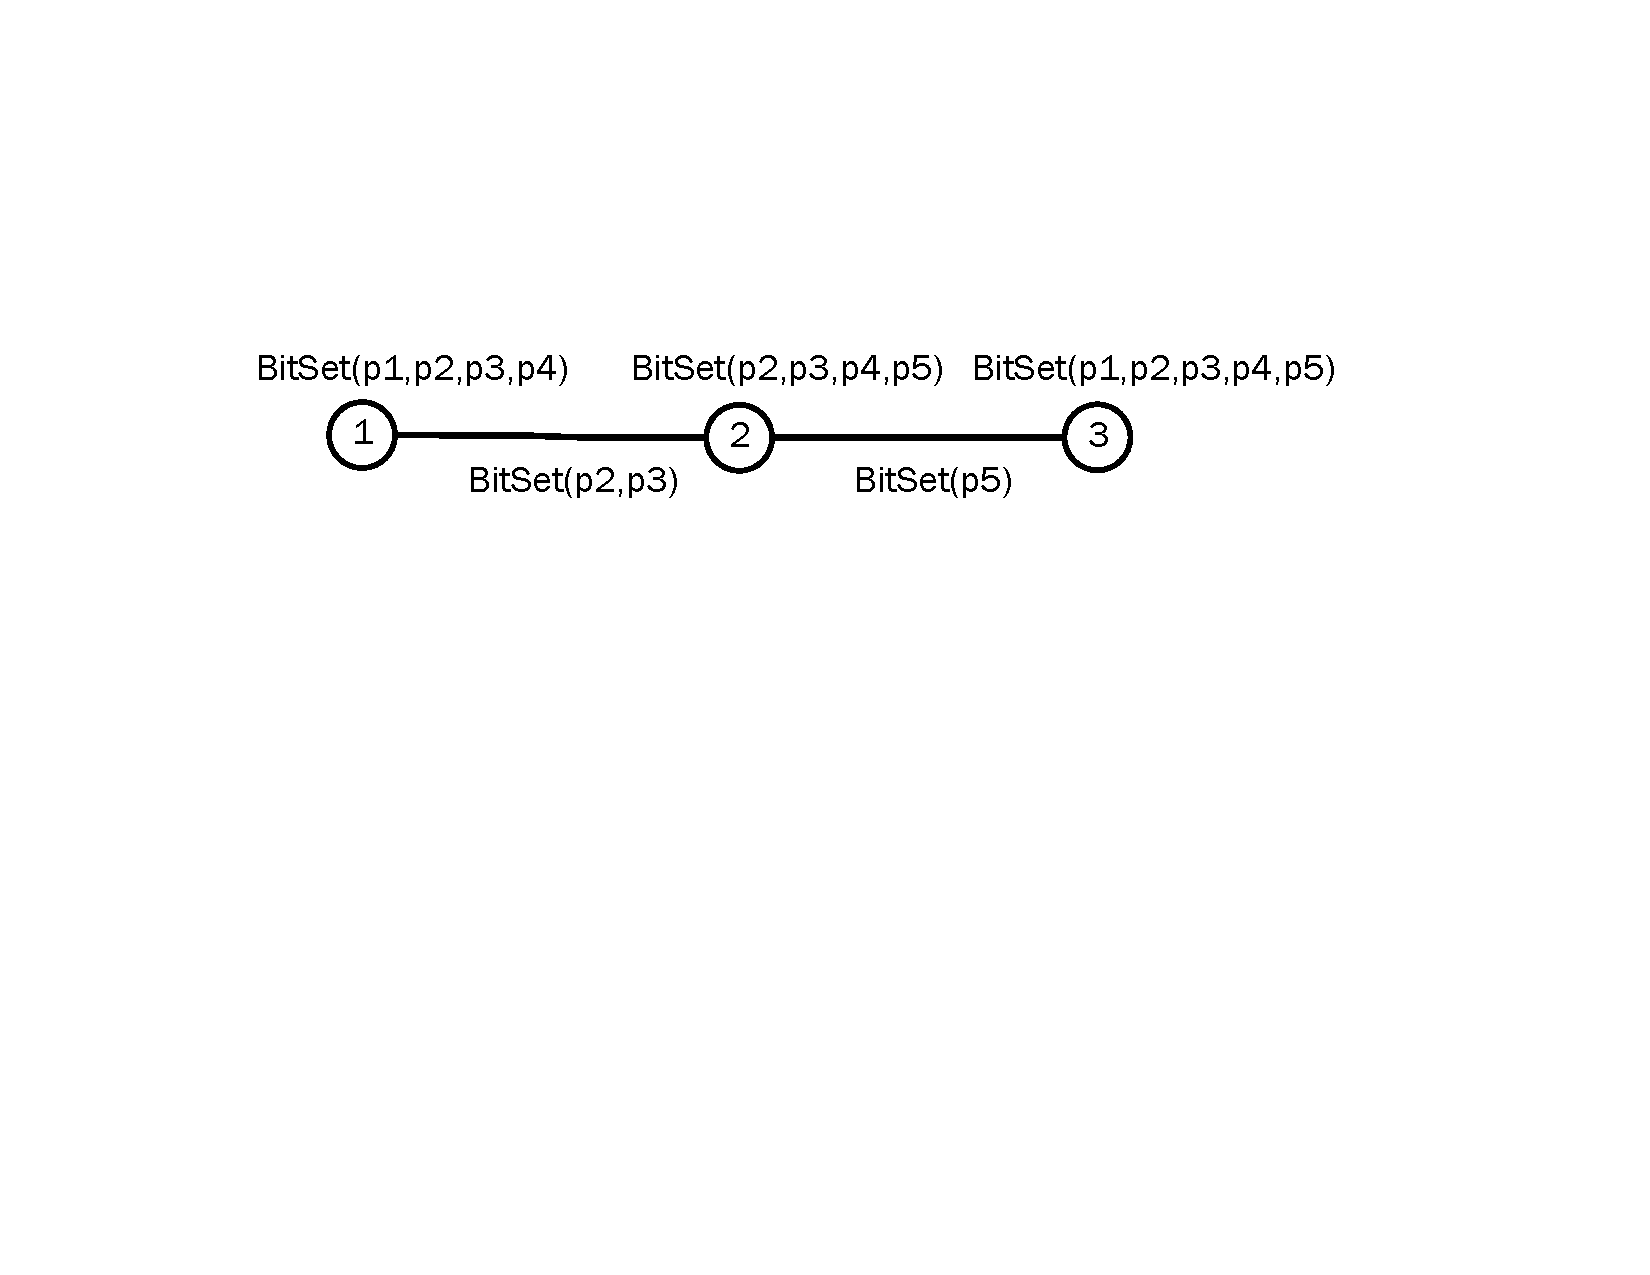
\includegraphics[width=3in]{figs/ogc.pdf}
\vspace{-0.2cm}
\caption{\og representation of \insql{T1}.}
\vspace{-0.1cm}
\label{fig:ogc}
\end{figure}

{\bf VertexEdge (VE)} is a direct implementation of the \tve model of
Definition~\ref{def:tg}, and is the most compact: one RDD contains all
vertices and another all edges.  Consistently with the GraphX API, all
vertex properties are stored together as a single nested attribute, as
are all edge properties.  We currently do not store the \tv and \te
relations separately but rather together with \tav and \tae,
respectively.  While VE does not necessitate a particular order of
tuples on disk, we opt for a physical layout in which all tuples
corresponding to the same vertex (resp. edge) are laid out
consecutively, and so VE preserves temporal locality.

\eat{ The main advantage of this schema-less attribute representation
  is that it can easily deal with schema evolution and leaves the
  details of attribute processing to the user. } 

VE supports all \tg algebra operations but cannot support analytics.
This is because an analytic is defined on a representative graph,
which VE does not materialize.  As we will show in
Section~\ref{sec:exp}, due to compactness this physical representation
is the most efficient for many operations.

{\bf OneGraph (OG)} is the most topologically compact representation,
which stores all vertices from \tav {\em and} edges from \tae once, in
a single data structure.  Information about time validity is stored
together with each vertex and edge.  Figure~\ref{fig:ogc} shows the OG
for \insql{T1} from Figure~\ref{fig:tg_rg}.  OG emphasizes temporal
locality, while also preserving structural locality, but leads to a
much denser graph than RG.  This, in turn, makes parallelizing
computation challenging.

An OG is implemented as a single GraphX graph.  To construct an \og
from \tve, vertices and edges of \tv and \te relations each are
grouped by key and mapped to bitsets, which in turn encode the
presence of a vertex or edge in each time period associated with some
representative graph of a \tg.  Because \og stores information only
about graph topology, far fewer periods must be represented and
computed for \og than for \rg.  The actual reduction depends on the
rate and nature of graph evolution.

As we will see experimentally in Section~\ref{sec:exp}, \og is often
the best-performing data structure for aggregation, and also has
competitive performance for analytics.  Because of this focus, \og
supports operations only on topology: analytics, aggregation. union,
and intersection for graphs with no vertex or edge attributes.  All
other operations are supported through inheritance from an abstract
parent, and are carried out on the VE data structure.  Thus \og and
\hg, below, can be thought of as indixes on VE.

{\bf HybridGraph (HG)} trades compactness of \og for better structural
locality of \rg, by aggregating together several consecutive
representative graphs, computing a single \og for each graph group,
and storing these as a parallel sequence.  In our current
implementation each \og in the sequence corresponds to the same number
of temporally adjacent graphs.
%
This is the simplest grouping method, and we observed that placing the
same number of graphs into each group often results in unbalanced
group sizes.  This is because evolving graphs commonly exhibit strong
temporal skew, with later graphs being significantly larger than earlier
ones.  We are currently working on more sophisticated grouping
approaches that would lead to better balance, and ultimately to better
performance.  However as we will see experimentally in
Section~\ref{sec:exp}, the current \hg implementation already improves
performance compared to \og, in some cases significantly.

Like \og, \hg focuses on topology-based analysis, and so does not
represent vertex and edge attributes. OG implements analytics,
aggregation, union, and intersection, and supports all other
operations through inheritance from VE.

\subsection{Additional Implementation Details}
\label{sec:sys:maint}

For the \trg logical representation, and for the physical
representations RG, OG and HG, we rely on GraphX to maintain valid
representative graphs, and so do not maintain referential integrity
explicitly.

  \eat{
    {\bf Foreign key constraint.}  The \ve data model includes a
    foreign key constraint from edges to vertices.  This constraint is
    naturally maintained by most operations while performing
    operations on V and E independently, as shown in
    Section~\ref{sec:algebra}.  For \insql{subgraph} and
    \insql{aggregate} additional steps are required to insure
    correctness.  We modify E tuples to enforce the foreign key
    constraint by joining on V, using either a broadcast or hash join
    depending on the size of V.  Each edge period is then modified to
    be the overlap of the periods of source and destination vertices
    and the original edge period.  Because this step is
    computationally expensive, it is only taken when necessary: when
    \insql{subgraph} has a predicate on V and when \insql{aggregate}
    has a higher level of quantification for V than for E.  GraphX
    graphs maintain foreign key constraint during subgraph operation
    and we make use of this for all representations besides VE.}

{\bf Partitioning.}  Graph partitioning has a tremendous impact on
performance.  A good partitioning strategy needs to be balanced,
assigning an approximately equal number of units to each partition,
and limit the number of cuts across partitions, reducing
cross-partition communication.  In our experiments we compare
performance with no repartitioning after load vs.  with
repartitioning, using the GraphX E2D edge partitioning strategy.  In
E2D, a sparse edge adjacency matrix is partitioned in two dimensions,
guaranteeing a $2 \sqrt{n}$ bound on vertex replication, where $n$ is
the number of partitions. E2D has been shown to provide good
performance for Pregel-style
analytics~\cite{DBLP:conf/osdi/GonzalezXDCFS14,MoffittTempWeb16}.

{\bf Graph loading.}  We use the Apache Parquet format for on-disk
storage, with one archive for vertices and another for edges,
temporally coalesced.  This format corresponds to the VE physical
representation~\ref{sec:sys:datastructs}.  In cases where there is no
more than 1 attribute per vertex and edge, this representation is also
the most compact.  \eat{If the input data is in uncoalesced snapshots,
  then it occupies space as a function of the graph evolution rate.}

For ease of use, we provide a GraphLoader utility that can initialize
any of the four physical representations of the \tg from Apache
Parquet files on HDFS or on local disk\eat{, provided that they follow
  the correct schema, using function call
  \insql{GraphLoader.loadDataParquet(\$path)}}.  The \ql user can also
implement custom graph loading methods to load vertices and edges, and
then use the \insql{fromRDDs} to initialize any of the four physical
representations.

\eat{ We have shown how our logical data model and semantics can be
  implemented in a distributed context. }  

\eat{Next, we show how different physical representations behave on each
operation of \tg algebra.}



